% !TeX root = ../main.tex
% Add the above to each chapter to make compiling the PDF easier in some editors.

\chapter{Results}\label{chapter:results}
In this chapter, the results of the in \autoref{sec:analysis-tools} computed experiments are
presented. Responses to the research questions are addressed in \autoref{sec:final_results}.
As previously described, three different video and image detection tools were used
to detect deepfakes. Calculations for the video detection tools were based on the
FaceForensics++ dataset, along with deepfake videos produced by DeepFaceLab and FaceSwap.
Image detection tools were evaluated using images created by FaceApp and Stable Diffusion,
as well as 20 authentic images.

\section{Comparative Results of tools}

\begin{figure}[htbp]
	\centering
	\begin{subfigure}{0.48\textwidth}
		\centering
		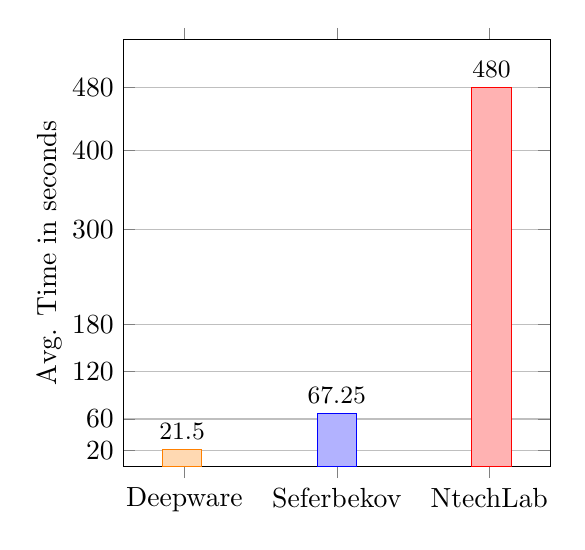
\begin{tikzpicture}
			\begin{axis}[
					ybar,
					bar width=5mm,
					width=7cm,
					height=7cm,
					enlarge x limits=0.2,
					legend style={at={(0.5,-0.2)},
							anchor=north,legend columns=-1},
					ylabel={Avg. Time in seconds},
					ylabel shift=-3pt,
					symbolic x coords={Deepware, Seferbekov, NtechLab},
					xtick={Deepware, Seferbekov, NtechLab},
					ytick={20,60,120,180,300,400,480},
					ymin=0,
					ymax=540,
					ymajorgrids=true,
					nodes near coords,
					every node near coord/.append style={font = {\fontsize{9 pt}{12 pt}\selectfont},color=black},
				]
				\addplot [orange,fill=orange!30,bar shift=-0.3mm] coordinates {(Deepware,21.5)};
				\addplot [blue,fill=blue!30] coordinates {(Seferbekov,67.25)};
				\addplot [red,fill=red!30, bar shift=0.3mm] coordinates {(NtechLab,480)};
			\end{axis}
		\end{tikzpicture}
		\caption{Video detection}
	\end{subfigure}
	\hfill
	\begin{subfigure}{0.48\textwidth}
		\centering
		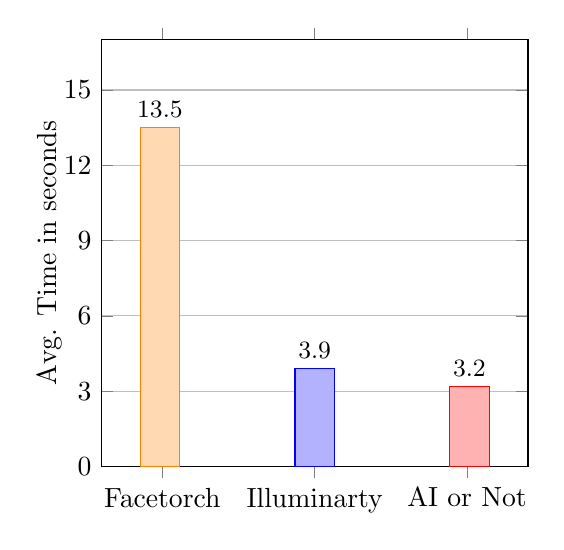
\begin{tikzpicture}
			\begin{axis}[
					ybar,
					bar width=5mm,
					width=7cm,
					height=7cm,
					enlarge x limits=0.2,
					legend style={at={(0.5,-0.2)},
							anchor=north,legend columns=-1},
					ylabel={Avg. Time in seconds},
					ylabel shift=-6pt,
					symbolic x coords={Facetorch, Illuminarty, AI or Not},
					xtick={Facetorch, Illuminarty, AI or Not},
					ytick={0,3,6,9,12,15},
					ymin=0,
					ymax=17,
					ymajorgrids=true,
					nodes near coords,
					every node near coord/.append style={font = {\fontsize{9 pt}{12 pt}\selectfont},color=black},
				]
				\addplot [orange,fill=orange!30,bar shift=-0.3mm] coordinates {(Facetorch,13.5)};
				\addplot [blue,fill=blue!30] coordinates {(Illuminarty,3.9)};
				\addplot [red,fill=red!30, bar shift=0.3mm] coordinates {(AI or Not,3.2)};
			\end{axis}
		\end{tikzpicture}
		\caption{Image detection}
	\end{subfigure}
	\caption{Comparison of the Processing Time of detection tools from~\autoref{sec:analysis-tools}}\label{fig:processing-time}
\end{figure}

From~\autoref{fig:processing-time}, it's evident that image detection tools process data faster
than video detection tools. This discrepancy is due to the nature of the tools:
image detection tools only process a single image (frame), whereas video detection tools may
need to break a video into numerous frames and analyze each one separately, which is considerably
more time-consuming. Additionally, among the video detection tools, NtechLab's tool was slower than
both Deepware and Seferbekov's tool. This might be because of the detection techniques they used.

The duration a tool takes to process data is tied to the size of the input. For instance,
Seferbekov's tool, when handling a video under 10MB, averaged a processing time of 20 seconds. However,
when confronted with a video exceeding 70MB, the time nearly tripled to almost a minute.
The size-to-time relationship is consistent across all tools, meaning the larger the size of the
input, the longer it's going to take the tool to process it.

A comparison of assessed metrics for video detection tools is displayed in~\autoref{fig:comparison_video}.
The comparison of which tool performed better is interesting. As we know, accuracy and precision
are defined as follows: Accuracy measures the fraction of all instances that are correctly
identified and precision measures the fraction of instances that were correctly predicted as
positive out of all predicted positives. So precision is especially important when the number
of false positives is high. In both of these cases, NtechLab performed better than the other two
tools. This is because NtechLab could detect more deepfakes.

Recall, also known as sensitivity, measures the proportion of actual positives that were
correctly identified. It is crucial when the cost of missing a positive instance is high.
And F-1 Score is a metric providing a balance between precision and recall, offering a more
comprehensive view of the performance. While NtechLab had higher accuracy and precision,
Deepware and Seferbekov's tool have caught up in terms of Recall and F1-Score. This suggests that
Deepware and Seferbekov's tool were more effective at correctly identifying true positive cases.

When it comes to image detection tools in~\autoref{fig:comparison_image}, AI or Not and
Illuminarty outperformed Facetorch. One possible reason could be that AI or Not and
Illuminarty are supported by companies and communities, receiving consistent updates.
On the other hand, Facetorch is an open-source project. It hasn't had any updates
since March 2023, which might make it less equipped to handle newer deepfake generation
techniques.

\begin{figure}[htbp]
	\centering
	\begin{subfigure}{0.48\textwidth}
		\centering
		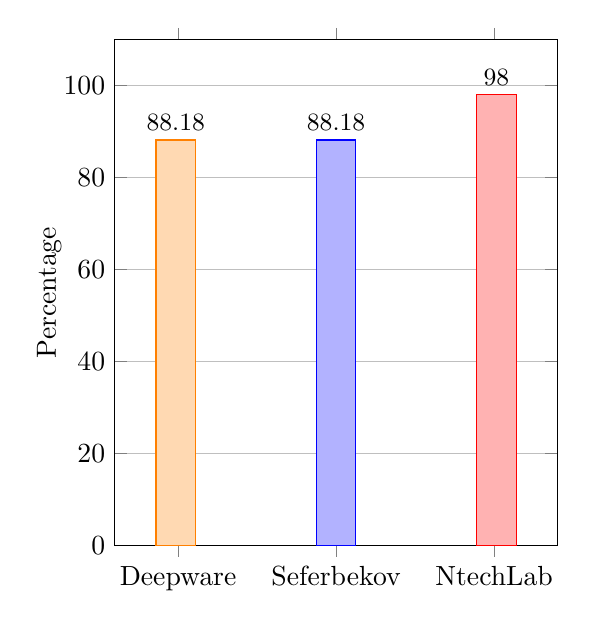
\begin{tikzpicture}
			\begin{axis}[
					ybar,
					bar width=5mm,
					width=7.2cm,
					height=8cm,
					enlarge x limits=0.2,
					legend style={at={(0.5,-0.2)},
							anchor=north,legend columns=-1},
					ylabel={Percentage},
					ylabel shift=-6pt,
					symbolic x coords={Deepware, Seferbekov, NtechLab},
					xtick={Deepware, Seferbekov, NtechLab},
					ytick={0,20,40,60,80,100},
					ymin=0,
					ymax=110,
					ymajorgrids=true,
					nodes near coords,
					every node near coord/.append style={font = {\fontsize{9 pt}{12 pt}\selectfont},color=black},
				]
				\addplot [orange,fill=orange!30,bar shift=-0.3mm] coordinates {(Deepware,88.18)};
				\addplot [blue,fill=blue!30] coordinates {(Seferbekov,88.18)};
				\addplot [red,fill=red!30, bar shift=0.3mm] coordinates {(NtechLab,98)};
			\end{axis}
		\end{tikzpicture}
		\caption{Detection accuracy}
	\end{subfigure}
	\hfill
	\begin{subfigure}{0.48\textwidth}
		\centering
		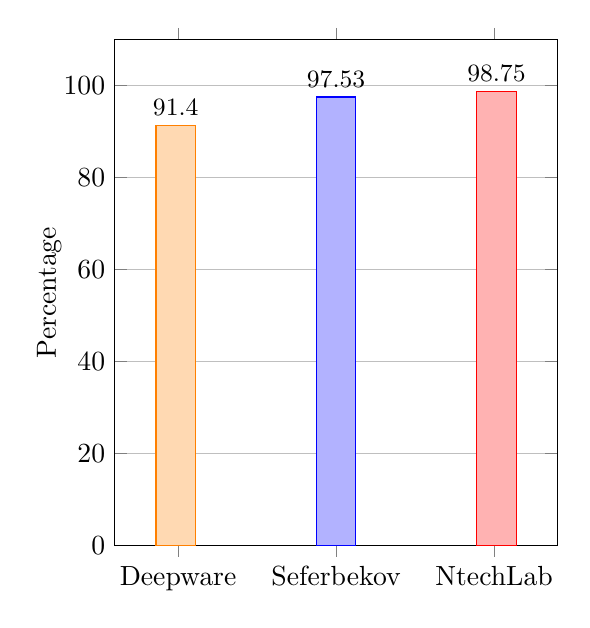
\begin{tikzpicture}
			\begin{axis}[
					ybar,
					bar width=5mm,
					width=7.2cm,
					height=8cm,
					enlarge x limits=0.2,
					legend style={at={(0.5,-0.2)},
							anchor=north,legend columns=-1},
					ylabel={Percentage},
					ylabel shift=-6pt,
					symbolic x coords={Deepware, Seferbekov, NtechLab},
					xtick={Deepware, Seferbekov, NtechLab},
					ytick={0,20,40,60,80,100},
					ymin=0,
					ymax=110,
					ymajorgrids=true,
					nodes near coords,
					every node near coord/.append style={font = {\fontsize{9 pt}{12 pt}\selectfont},color=black},
				]
				\addplot [orange,fill=orange!30,bar shift=-0.3mm] coordinates {(Deepware,91.40)};
				\addplot [blue,fill=blue!30] coordinates {(Seferbekov,97.53)};
				\addplot [red,fill=red!30, bar shift=0.3mm] coordinates {(NtechLab,98.75)};
			\end{axis}
		\end{tikzpicture}
		\caption{Precision}
	\end{subfigure}

	\vspace{0.5cm}

	\begin{subfigure}{0.48\textwidth}
		\centering
		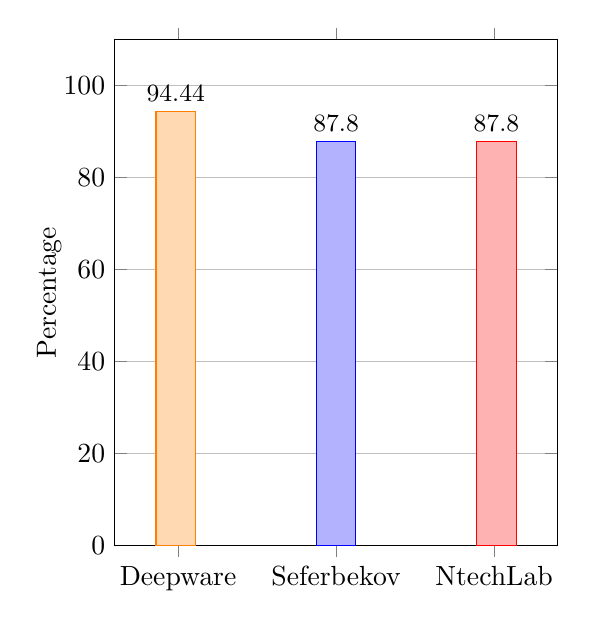
\begin{tikzpicture}
			\begin{axis}[
					ybar,
					bar width=5mm,
					width=7.2cm,
					height=8cm,
					enlarge x limits=0.2,
					legend style={at={(0.5,-0.2)},
							anchor=north,legend columns=-1},
					ylabel={Percentage},
					ylabel shift=-6pt,
					symbolic x coords={Deepware, Seferbekov, NtechLab},
					xtick={Deepware, Seferbekov, NtechLab},
					ytick={0,20,40,60,80,100},
					ymin=0,
					ymax=110,
					ymajorgrids=true,
					nodes near coords,
					every node near coord/.append style={font = {\fontsize{9 pt}{12 pt}\selectfont},color=black},
				]
				\addplot [orange,fill=orange!30,bar shift=-0.3mm] coordinates {(Deepware,94.44)};
				\addplot [blue,fill=blue!30] coordinates {(Seferbekov,87.8)};
				\addplot [red,fill=red!30, bar shift=0.3mm] coordinates {(NtechLab,87.8)};
			\end{axis}
		\end{tikzpicture}
		\caption{Recall}
	\end{subfigure}
	\hfill
	\begin{subfigure}{0.48\textwidth}
		\centering
		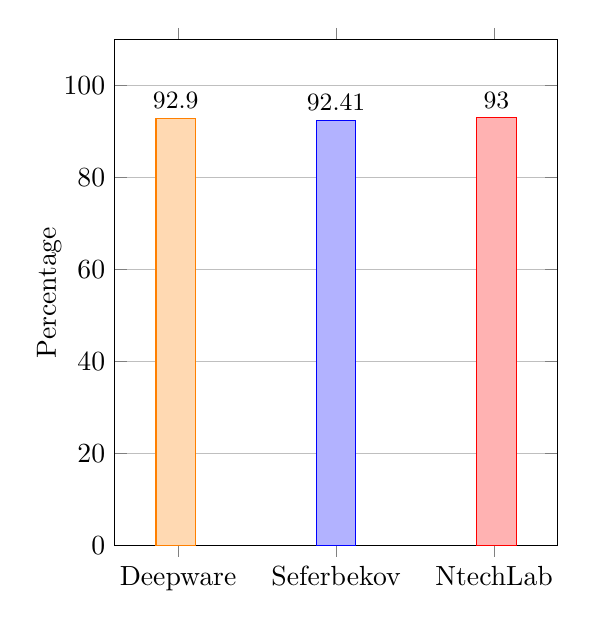
\begin{tikzpicture}
			\begin{axis}[
					ybar,
					bar width=5mm,
					width=7.2cm,
					height=8cm,
					enlarge x limits=0.2,
					legend style={at={(0.5,-0.2)},
							anchor=north,legend columns=-1},
					ylabel={Percentage},
					ylabel shift=-6pt,
					symbolic x coords={Deepware, Seferbekov, NtechLab},
					xtick={Deepware, Seferbekov, NtechLab},
					ytick={0,20,40,60,80,100},
					ymin=0,
					ymax=110,
					ymajorgrids=true,
					nodes near coords,
					every node near coord/.append style={font = {\fontsize{9 pt}{12 pt}\selectfont},color=black},
				]
				\addplot [orange,fill=orange!30,bar shift=-0.3mm] coordinates {(Deepware,92.9)};
				\addplot [blue,fill=blue!30] coordinates {(Seferbekov,92.41)};
				\addplot [red,fill=red!30, bar shift=0.3mm] coordinates {(NtechLab,93)};
			\end{axis}
		\end{tikzpicture}
		\caption{F1-Score}
	\end{subfigure}
	\caption{Comparison of video detection tools from~\autoref{sec:analysis-tools} according
		to the evaluation metrics listed in~\autoref{tab:evaluation_metrics}}\label{fig:comparison_video}
\end{figure}


\begin{figure}[htbp]
	\centering
	\begin{subfigure}{0.48\textwidth}
		\centering
		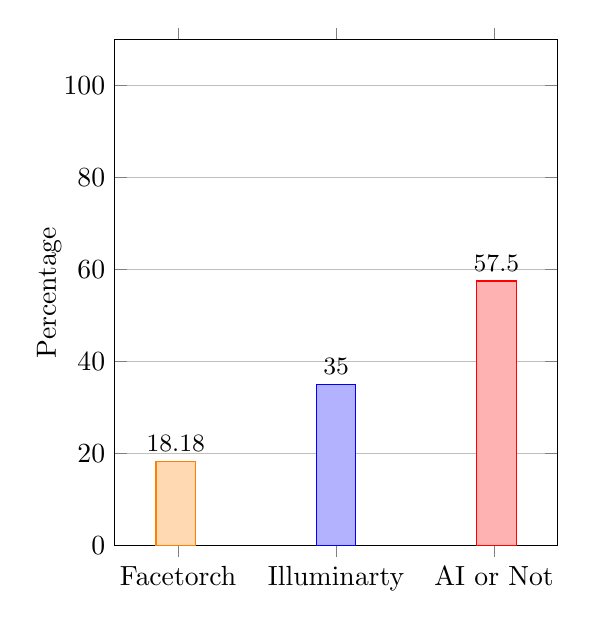
\begin{tikzpicture}
			\begin{axis}[
					ybar,
					bar width=5mm,
					width=7.2cm,
					height=8cm,
					enlarge x limits=0.2,
					legend style={at={(0.5,-0.2)},
							anchor=north,legend columns=-1},
					ylabel={Percentage},
					ylabel shift=-6pt,
					symbolic x coords={Facetorch, Illuminarty, AI or Not},
					xtick={Facetorch, Illuminarty, AI or Not},
					ytick={0,20,40,60,80,100},
					ymin=0,
					ymax=110,
					ymajorgrids=true,
					nodes near coords,
					every node near coord/.append style={font = {\fontsize{9 pt}{12 pt}\selectfont},color=black},
				]
				\addplot [orange,fill=orange!30,bar shift=-0.3mm] coordinates {(Facetorch,18.18)};
				\addplot [blue,fill=blue!30] coordinates {(Illuminarty,35)};
				\addplot [red,fill=red!30, bar shift=0.3mm] coordinates {(AI or Not,57.5)};
			\end{axis}
		\end{tikzpicture}
		\caption{Detection accuracy}
	\end{subfigure}
	\hfill
	\begin{subfigure}{0.48\textwidth}
		\centering
		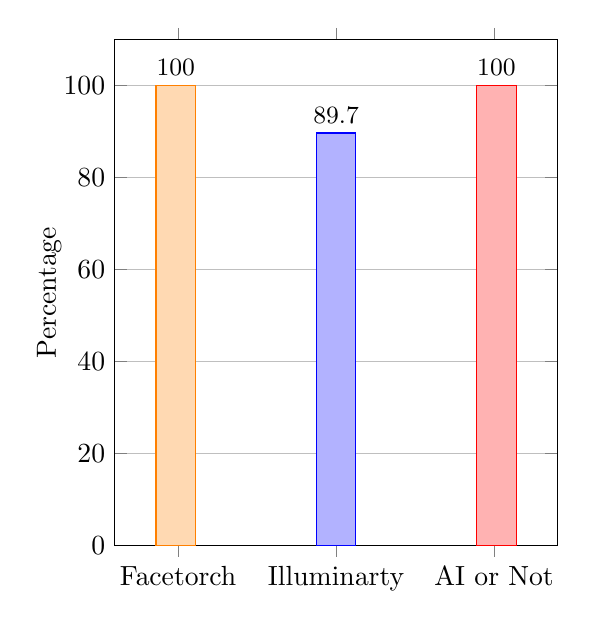
\begin{tikzpicture}
			\begin{axis}[
					ybar,
					bar width=5mm,
					width=7.2cm,
					height=8cm,
					enlarge x limits=0.2,
					legend style={at={(0.5,-0.2)},
							anchor=north,legend columns=-1},
					ylabel={Percentage},
					ylabel shift=-6pt,
					symbolic x coords={Facetorch, Illuminarty, AI or Not},
					xtick={Facetorch, Illuminarty, AI or Not},
					ytick={0,20,40,60,80,100},
					ymin=0,
					ymax=110,
					ymajorgrids=true,
					nodes near coords,
					every node near coord/.append style={font = {\fontsize{9 pt}{12 pt}\selectfont},color=black},
				]
				\addplot [orange,fill=orange!30,bar shift=-0.3mm] coordinates {(Facetorch,100)};
				\addplot [blue,fill=blue!30] coordinates {(Illuminarty,89.7)};
				\addplot [red,fill=red!30, bar shift=0.3mm] coordinates {(AI or Not,100)};
			\end{axis}
		\end{tikzpicture}
		\caption{Precision}
	\end{subfigure}

	\vspace{0.5cm}

	\begin{subfigure}{0.48\textwidth}
		\centering
		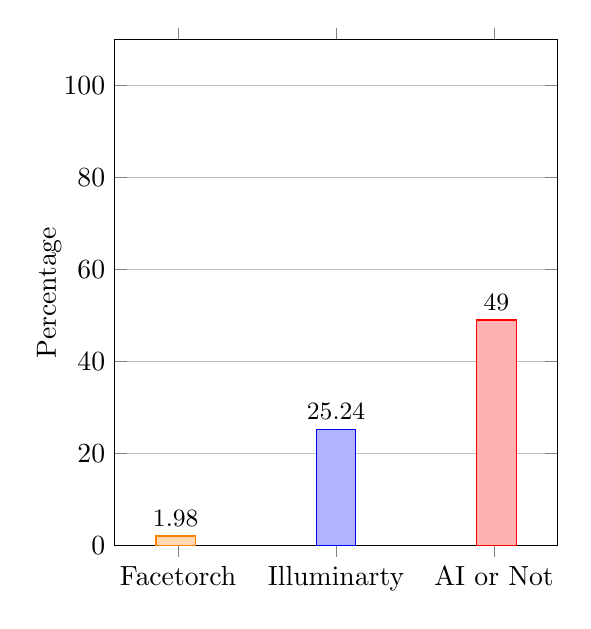
\begin{tikzpicture}
			\begin{axis}[
					ybar,
					bar width=5mm,
					width=7.2cm,
					height=8cm,
					enlarge x limits=0.2,
					legend style={at={(0.5,-0.2)},
							anchor=north,legend columns=-1},
					ylabel={Percentage},
					ylabel shift=-6pt,
					symbolic x coords={Facetorch, Illuminarty, AI or Not},
					xtick={Facetorch, Illuminarty, AI or Not},
					ytick={0,20,40,60,80,100},
					ymin=0,
					ymax=110,
					ymajorgrids=true,
					nodes near coords,
					every node near coord/.append style={font = {\fontsize{9 pt}{12 pt}\selectfont},color=black},
				]
				\addplot [orange,fill=orange!30,bar shift=-0.3mm] coordinates {(Facetorch,1.98)};
				\addplot [blue,fill=blue!30] coordinates {(Illuminarty,25.24)};
				\addplot [red,fill=red!30, bar shift=0.3mm] coordinates {(AI or Not,49)};
			\end{axis}
		\end{tikzpicture}
		\caption{Recall}
	\end{subfigure}
	\hfill
	\begin{subfigure}{0.48\textwidth}
		\centering
		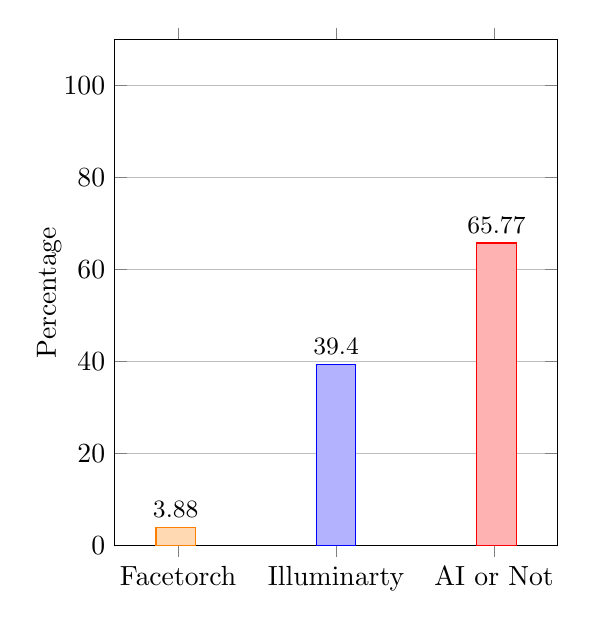
\begin{tikzpicture}
			\begin{axis}[
					ybar,
					bar width=5mm,
					width=7.2cm,
					height=8cm,
					enlarge x limits=0.2,
					legend style={at={(0.5,-0.2)},
							anchor=north,legend columns=-1},
					ylabel={Percentage},
					ylabel shift=-6pt,
					symbolic x coords={Facetorch, Illuminarty, AI or Not},
					xtick={Facetorch, Illuminarty, AI or Not},
					ytick={0,20,40,60,80,100},
					ymin=0,
					ymax=110,
					ymajorgrids=true,
					nodes near coords,
					every node near coord/.append style={font = {\fontsize{9 pt}{12 pt}\selectfont},color=black},
				]
				\addplot [orange,fill=orange!30,bar shift=-0.3mm] coordinates {(Facetorch,3.88)};
				\addplot [blue,fill=blue!30] coordinates {(Illuminarty,39.4)};
				\addplot [red,fill=red!30, bar shift=0.3mm] coordinates {(AI or Not,65.77)};
			\end{axis}
		\end{tikzpicture}
		\caption{F1-Score}
	\end{subfigure}
	\caption{Comparison of image detection tools from~\autoref{sec:analysis-tools} according
		to the evaluation metrics listed in~\autoref{tab:evaluation_metrics}}\label{fig:comparison_image}
\end{figure}

\section{Final Results}\label{sec:final_results}
To conclude the achieved results, it's noticeable that some tools might have a high accuracy rate
but perform poorly in terms of recall and F1-Score. Contrarily, certain tools might demonstrate
high precision but low recall, which might indicate that the tool misses some actual
positives. By comparing these metrics across the testes tools, a clearer insight into their
strengths and limitations can be gained. This, in turn, helps us make important decisions on
which tool is ideal for a particular task.

An overview of selection criteria and evaluation metrics discussed in \autoref{tab:selection_criteria}
and \autoref{tab:evaluation_metrics} for Deepware is provided in \autoref{tab:deepware-overview}, for Seferbekov in \autoref{tab:seferbekov-overview},
for NtechLab in \autoref{tab:ntechlab-overview}, for Facetorch in \autoref{tab:facetorch-overview},
for Illuminarty in \autoref{tab:illuminarty-overview}, for AI or Not in \autoref{tab:ai-or-not-overview}.

\subsection{Research Questions}
\textit{To answer \ac{RQ}1:} Through various tests with each deepfake detection tool,
comparative results were obtained. From this analysis, it became evident which tools were more
user-friendly than others. Overall, tools such as Deepware, AI or Not and Illuminarty stood out
as particularly accessible and straightforward. Even for individuals without any prior knowledge
of deepfakes and their detection, these tools proved effective in quickly identifying deepfakes.
However, while some tools like the one offered by NTechLab or Seferbekov are open-source and
integrate with platforms like Hugging Face and Google Colab, their ease of use might still pose
challenges for novices. The presence of documentation, user interfaces, and community support
can enhance user-friendliness, but there remains a potential learning curve for those unfamiliar
with the field.

\textit{To answer \ac{RQ}2:} In evaluating the effectiveness of the selected deepfake detection
tools, there were notable disparities in their performance. For instance, Facetorch, while
promising in its approach, showed limitations in consistently identifying forgeries,
especially when confronted with sophisticated deepfake generation techniques such as FaceApp
and StableDiffusion. On the other hand, video detection tools demonstrated a higher precision
rate. For example, when testing against deepfakes generated using DeepFaceLab, the video
detection tools were able to discern the forgeries with a higher accuracy rate compared to
tools that primarily focused on images. This suggests that while some tools are advancing
in their detection capabilities, there remains a spectrum of effectiveness, and the choice
of tool should be contingent on the specific type of media (image or video) being analyzed.

Furthermore, the choice of a dataset for training and testing these tools plays a pivotal role
in their effectiveness. A tool trained on an outdated or narrow dataset might not perform as
well when exposed to deepfakes created with the latest techniques. This underscores the
importance of regularly updating detection tools and ensuring they are trained on diverse
and current datasets.

\textit{To answer \ac{RQ}3:} In addressing Research Question 3, the privacy policies
and practices of the selected deepfake detection tools were examined. The goal was to
discern how user data, especially sensitive content uploaded for deepfake detection,
was handled, stored, and potentially shared.

It was found that while tools like Deepware, Illuminarty and AI or Not provided clear privacy
policies, others were not transparent about their data practices. The lack of a privacy
policy can lead to concerns about potential unauthorized data sharing or misuse.

The importance of understanding these privacy implications stems from the need to
ensure that user content is not misused and that tools comply with global data privacy
regulations like \ac{GDPR}.


\setlist[itemize]{nosep, left=0em, before=\vspace{-0.6\baselineskip}, after=\vspace{-0.6\baselineskip}}
\begin{table}[htpb]
	\caption{Overview of selection criteria and evaluation metrics for Deepware}\label{tab:deepware-overview}
	\centering
	\small
	\begin{tabularx}{\textwidth}{l X}
		\toprule
		\textbf{Criteria \& Metrics} & \textbf{Evaluation}                                        \\
		\midrule
		Ease of Use and Limitations  & \begin{itemize}
			                               \item Doesn't require local installation
			                               \item Provides \ac{API} access
			                               \item Lack of updates since 2021
		                               \end{itemize}                    \\
		\addlinespace
		Accessibility                & \begin{itemize}
			                               \item Accessible through: \url{https://deepware.ai/}
			                               \item Proprietary
			                               \item No Hugging Face Space or Google Colab available
		                               \end{itemize}       \\
		\addlinespace
		Support and Documentation    & \begin{itemize}
			                               \item No User Documentation
			                               \item Provides FAQ section: \url{https://deepware.ai/faq/}
		                               \end{itemize}  \\
		\addlinespace
		Difficulty of Use            & \begin{itemize}
			                               \item Easy
		                               \end{itemize}                                             \\
		\addlinespace
		Cost considerations          & \begin{itemize}
			                               \item Free
		                               \end{itemize}                                             \\
		\addlinespace
		Privacy Policy               & \begin{itemize}
			                               \item Website operation: Zemana owns and runs Deepware
			                               \item Data Collection: Gathers personal and usage data
			                               \item Data Usage: For service improvement and notifications
			                               \item Data Disclosure: Shared for specific purposes
			                               \item User Rights: Access and modify personal data
		                               \end{itemize} \\
		\addlinespace
		Interpretability             & \begin{itemize}
			                               \item Results are given as deepfake likelihood percentages
		                               \end{itemize}  \\
		\addlinespace
		Dataset Compatibility        & \begin{itemize}
			                               \item No incompatible dataset was found for this tool
		                               \end{itemize}       \\
		\addlinespace
		Training Models              & \begin{itemize}
			                               \item Avatarify
			                               \item Deepware's model
			                               \item Seferbekov
			                               \item Ensemble
		                               \end{itemize}                                      \\
		\addlinespace
		Programming Language         & \begin{itemize}
			                               \item Python
		                               \end{itemize}                                             \\
		\bottomrule
	\end{tabularx}
\end{table}

\begin{table}[htpb]
	\caption{Overview of selection criteria and evaluation metrics for Seferbekov's tool}\label{tab:seferbekov-overview}
	\centering
	\small
	\begin{tabularx}{\textwidth}{l X}
		\toprule
		\textbf{Criteria \& Metrics} & \textbf{Evaluation}                                                                \\
		\midrule
		Ease of Use and Limitations  & \begin{itemize}
			                               \item Requires local installation for development
			                               \item No \ac{API} access
			                               \item Lack of updates since 2021
			                               \item Requires better hardware and \ac{GPU}
		                               \end{itemize}                                   \\
		\addlinespace
		Accessibility                & \begin{itemize}
			                               \item Accessible through: \url{https://github.com/selimsef/dfdc_deepfake_challenge}
			                               \item Open source
			                               \item Integration with Hugging Face and Google Colab possible
		                               \end{itemize} \\
		Support and Documentation    & \begin{itemize}
			                               \item No active support and usage documentation
			                               \item Documentation for development available
		                               \end{itemize}                                     \\
		\addlinespace
		Difficulty of Use            & \begin{itemize}
			                               \item Challenging
		                               \end{itemize}                                                                   \\
		\addlinespace
		Cost considerations          & \begin{itemize}
			                               \item Free
		                               \end{itemize}                                                                     \\
		\addlinespace
		Privacy Policy               & \begin{itemize}
			                               \item No Privacy Policy available
		                               \end{itemize}                                                   \\
		\addlinespace
		Interpretability             & \begin{itemize}
			                               \item Results are given as deepfake likelihood percentages in a \ac{CSV} file
		                               \end{itemize}       \\
		\addlinespace
		Dataset Compatibility        & \begin{itemize}
			                               \item No incompatible dataset was found for this tool
		                               \end{itemize}                               \\
		\addlinespace
		Training Models              & \begin{itemize}
			                               \item EfficientNet B7 models
		                               \end{itemize}                                                        \\
		\addlinespace
		Programming Language         & \begin{itemize}
			                               \item Python
		                               \end{itemize}                                                                     \\
		\bottomrule
	\end{tabularx}
\end{table}

\begin{table}[htpb]
	\caption{Overview of selection criteria and evaluation metrics for NtechLab's tool}\label{tab:ntechlab-overview}
	\centering
	\small
	\begin{tabularx}{\textwidth}{l X}
		\toprule
		\textbf{Criteria \& Metrics} & \textbf{Evaluation}                                                                              \\
		\midrule
		Ease of Use and Limitations  & \begin{itemize}
			                               \item Requires local installation for development
			                               \item No \ac{API} access
			                               \item Lack of updates since 2020
			                               \item Requires better hardware and \ac{GPU}
		                               \end{itemize}                                                 \\
		\addlinespace
		Accessibility                & \begin{itemize}
			                               \item Accessible through:\newline \url{https://github.com/NTech-Lab/deepfake-detection-challenge}
			                               \item Open source
			                               \item Integration with Hugging Face and Google Colab\newline possible
		                               \end{itemize} \\\addlinespace

		Support and Documentation    & \begin{itemize}
			                               \item No active support and usage documentation
			                               \item Documentation for development available
		                               \end{itemize}                                                   \\
		\addlinespace
		Difficulty of Use            & \begin{itemize}
			                               \item Challenging
		                               \end{itemize}                                                                                 \\
		\addlinespace
		Cost considerations          & \begin{itemize}
			                               \item Free
		                               \end{itemize}                                                                                   \\
		\addlinespace
		Privacy Policy               & \begin{itemize}
			                               \item No Privacy Policy available
		                               \end{itemize}                                                                 \\
		\addlinespace
		Interpretability             & \begin{itemize}
			                               \item Results are given as deepfake likelihood\newline percentages in a \ac{CSV} file
		                               \end{itemize}             \\
		\addlinespace
		Dataset Compatibility        & \begin{itemize}
			                               \item No incompatible dataset was found for this tool
		                               \end{itemize}                                             \\
		\addlinespace
		Training Models              & \begin{itemize}
			                               \item EfficientNet B7 Noisy Student pre-trained models
		                               \end{itemize}                                            \\
		\addlinespace
		Programming Language         & \begin{itemize}
			                               \item Python
		                               \end{itemize}                                                                                   \\
		\bottomrule
	\end{tabularx}
\end{table}

\begin{table}[htpb]
	\caption{Overview of selection criteria and evaluation metrics for Facetorch}\label{tab:facetorch-overview}
	\centering
	\small
	\begin{tabularx}{\textwidth}{l X}
		\toprule
		\textbf{Criteria \& Metrics} & \textbf{Evaluation}                                                                \\
		\midrule
		Ease of Use and Limitations  & \begin{itemize}
			                               \item Requires local installation for development
			                               \item No \ac{API} access
			                               \item Has some inconsistencies detecting deepfakes
			                               \item Requires better hardware and \ac{GPU}
		                               \end{itemize}                                  \\
		\addlinespace
		Accessibility                & \begin{itemize}
			                               \item Accessible through:\newline \url{https://github.com/tomas-gajarsky/facetorch}
			                               \item Open source
			                               \item Hugging Face Space and Google Colab available
		                               \end{itemize} \\
		\addlinespace
		Support and Documentation    & \begin{itemize}
			                               \item User Guide and Documentation available
			                               \item Documentation for development available
			                               \item Disclaimer of not perfect results from developer
		                               \end{itemize}                              \\
		\addlinespace
		Difficulty of Use            & \begin{itemize}
			                               \item Moderate
		                               \end{itemize}                                                                     \\
		\addlinespace
		Cost considerations          & \begin{itemize}
			                               \item Free
		                               \end{itemize}                                                                     \\
		\addlinespace
		Privacy Policy               & \begin{itemize}
			                               \item Developer's warning to \cite{facetorch-privacy} regarding tool usage.
		                               \end{itemize}         \\
		\addlinespace
		Interpretability             & \begin{itemize}
			                               \item Results are labeled as `Fake' or `Real'
		                               \end{itemize}                                       \\
		\addlinespace
		Dataset Compatibility        & \begin{itemize}
			                               \item Problems detecting FaceApp and StableDiffusion deepfakes
		                               \end{itemize}                      \\
		\addlinespace
		Training Models              & \begin{itemize}
			                               \item Face Detection~\cite{Deng_2020_CVPR}
			                               \item Facial Representation Learning~\cite{bulat2022pretraining}
			                               \item Face Verification~\cite{jung2022unified,kim2023adaface}
			                               \item Facial Expression Recognition~\cite{9582508}
			                               \item Deepfake Detection~\cite{Luo_2022,seferbekov-github}
			                               \item 3D Face Alignment~\cite{wu2021synergy}
		                               \end{itemize}                    \\
		\addlinespace
		Programming Language         & \begin{itemize}
			                               \item Python and Pytorch
		                               \end{itemize}                                                            \\
		\bottomrule
	\end{tabularx}
\end{table}

\begin{table}[htpb]
	\caption{Overview of selection criteria and evaluation metrics for Illuminarty}\label{tab:illuminarty-overview}
	\centering
	\small
	\begin{tabularx}{\textwidth}{l X}
		\toprule
		\textbf{Criteria \& Metrics} & \textbf{Evaluation}                                        \\
		\midrule
		Ease of Use and Limitations  & \begin{itemize}
			                               \item Doesn't require local installation
			                               \item Provides \ac{API} access
		                               \end{itemize}                    \\
		\addlinespace
		Accessibility                & \begin{itemize}
			                               \item Accessible through: \url{https://app.illuminarty.ai/}
			                               \item Proprietary
			                               \item No Hugging Face or Google Colab available
		                               \end{itemize} \\
		\addlinespace
		Support and Documentation    & \begin{itemize}
			                               \item Active support available
			                               \item No documentation
		                               \end{itemize}                              \\
		\addlinespace
		Difficulty of Use            & \begin{itemize}
			                               \item Easy
		                               \end{itemize}                                             \\
		\addlinespace
		Cost considerations          & \begin{itemize}
			                               \item Free and Paid versions available
		                               \end{itemize}                      \\
		\addlinespace
		Privacy Policy               & \begin{itemize}
			                               \item Processing: Only voluntary data used.
			                               \item Payments: Secure transaction methods.
			                               \item Data Collection: Temporary image retention.
			                               \item Policy Changes: Updates at discretion.
		                               \end{itemize}           \\
		\addlinespace
		Interpretability             & \begin{itemize}
			                               \item Results are given as deepfake likelihood percentages
		                               \end{itemize}  \\
		\addlinespace
		Dataset Compatibility        & \begin{itemize}
			                               \item Has some problems detecting FaceApp deepfakes
		                               \end{itemize}         \\
		\addlinespace
		Training Models              & \begin{itemize}
			                               \item No available information
		                               \end{itemize}                              \\
		\addlinespace
		Programming Language         & \begin{itemize}
			                               \item No available information
		                               \end{itemize}                              \\
		\bottomrule
	\end{tabularx}
\end{table}

\begin{table}[htpb]
	\caption{Overview of selection criteria and evaluation metrics for AI or Not}\label{tab:ai-or-not-overview}
	\centering
	\small
	\begin{tabularx}{\textwidth}{l X}
		\toprule
		\textbf{Criteria \& Metrics} & \textbf{Evaluation}                                                   \\
		\midrule
		Ease of Use and Limitations  & \begin{itemize}
			                               \item Doesn't require local installation
			                               \item Provides \ac{API} access
			                               \item Provides Browser extension and Telegram bot
		                               \end{itemize}                      \\
		\addlinespace
		Accessibility                & \begin{itemize}
			                               \item Accessible through: \url{https://www.aiornot.com/}
			                               \item Proprietary
			                               \item No Hugging Face or Google Colab available
		                               \end{itemize}               \\
		\addlinespace
		Support and Documentation    & \begin{itemize}
			                               \item Active support, documentation and FAQ available
		                               \end{itemize}                  \\
		\addlinespace
		Difficulty of Use            & \begin{itemize}
			                               \item Easy
		                               \end{itemize}                                                        \\
		\addlinespace
		Cost considerations          & \begin{itemize}
			                               \item Free and Paid versions available
		                               \end{itemize}                                 \\
		\addlinespace
		Privacy Policy               & \begin{itemize}
			                               \item Data Collection: Gathering diverse user data.
			                               \item Use of Data: Service improvement and marketing.
			                               \item Data Sharing: Third-party involvement.
			                               \item About \& Consent: Agreeing to data practices.
			                               \item User Rights: State-specific privacy rights.
		                               \end{itemize}                  \\
		\addlinespace
		Interpretability             & \begin{itemize}
			                               \item Results are given as deepfake likelihood percentages
		                               \end{itemize}             \\
		\addlinespace
		Dataset Compatibility        & \begin{itemize}
			                               \item Compatible with StableDiffusion, MidJourney, DALL-E and \ac{GAN}
		                               \end{itemize} \\
		\addlinespace
		Training Models              & \begin{itemize}
			                               \item No available information
		                               \end{itemize}                                         \\
		\addlinespace
		Programming Language         & \begin{itemize}
			                               \item No available information
		                               \end{itemize}                                         \\
		\bottomrule
	\end{tabularx}
\end{table}